\documentclass{article}

\usepackage{graphicx}
\usepackage{tikz}
\usepackage{tikzsymbols}
\usetikzlibrary{calc,patterns,shapes.geometric}
\pagestyle{empty}
\usepackage[margin=0pt]{geometry}
\geometry{papersize={14in,12in}}

\def\centerarc[#1](#2)(#3:#4:#5){\draw[#1] ($(#2)+({#5*cos(#3)},{#5*sin(#3)})$) arc (#3:#4:#5);}

\begin{document}
	\begin{figure}
		\centering
		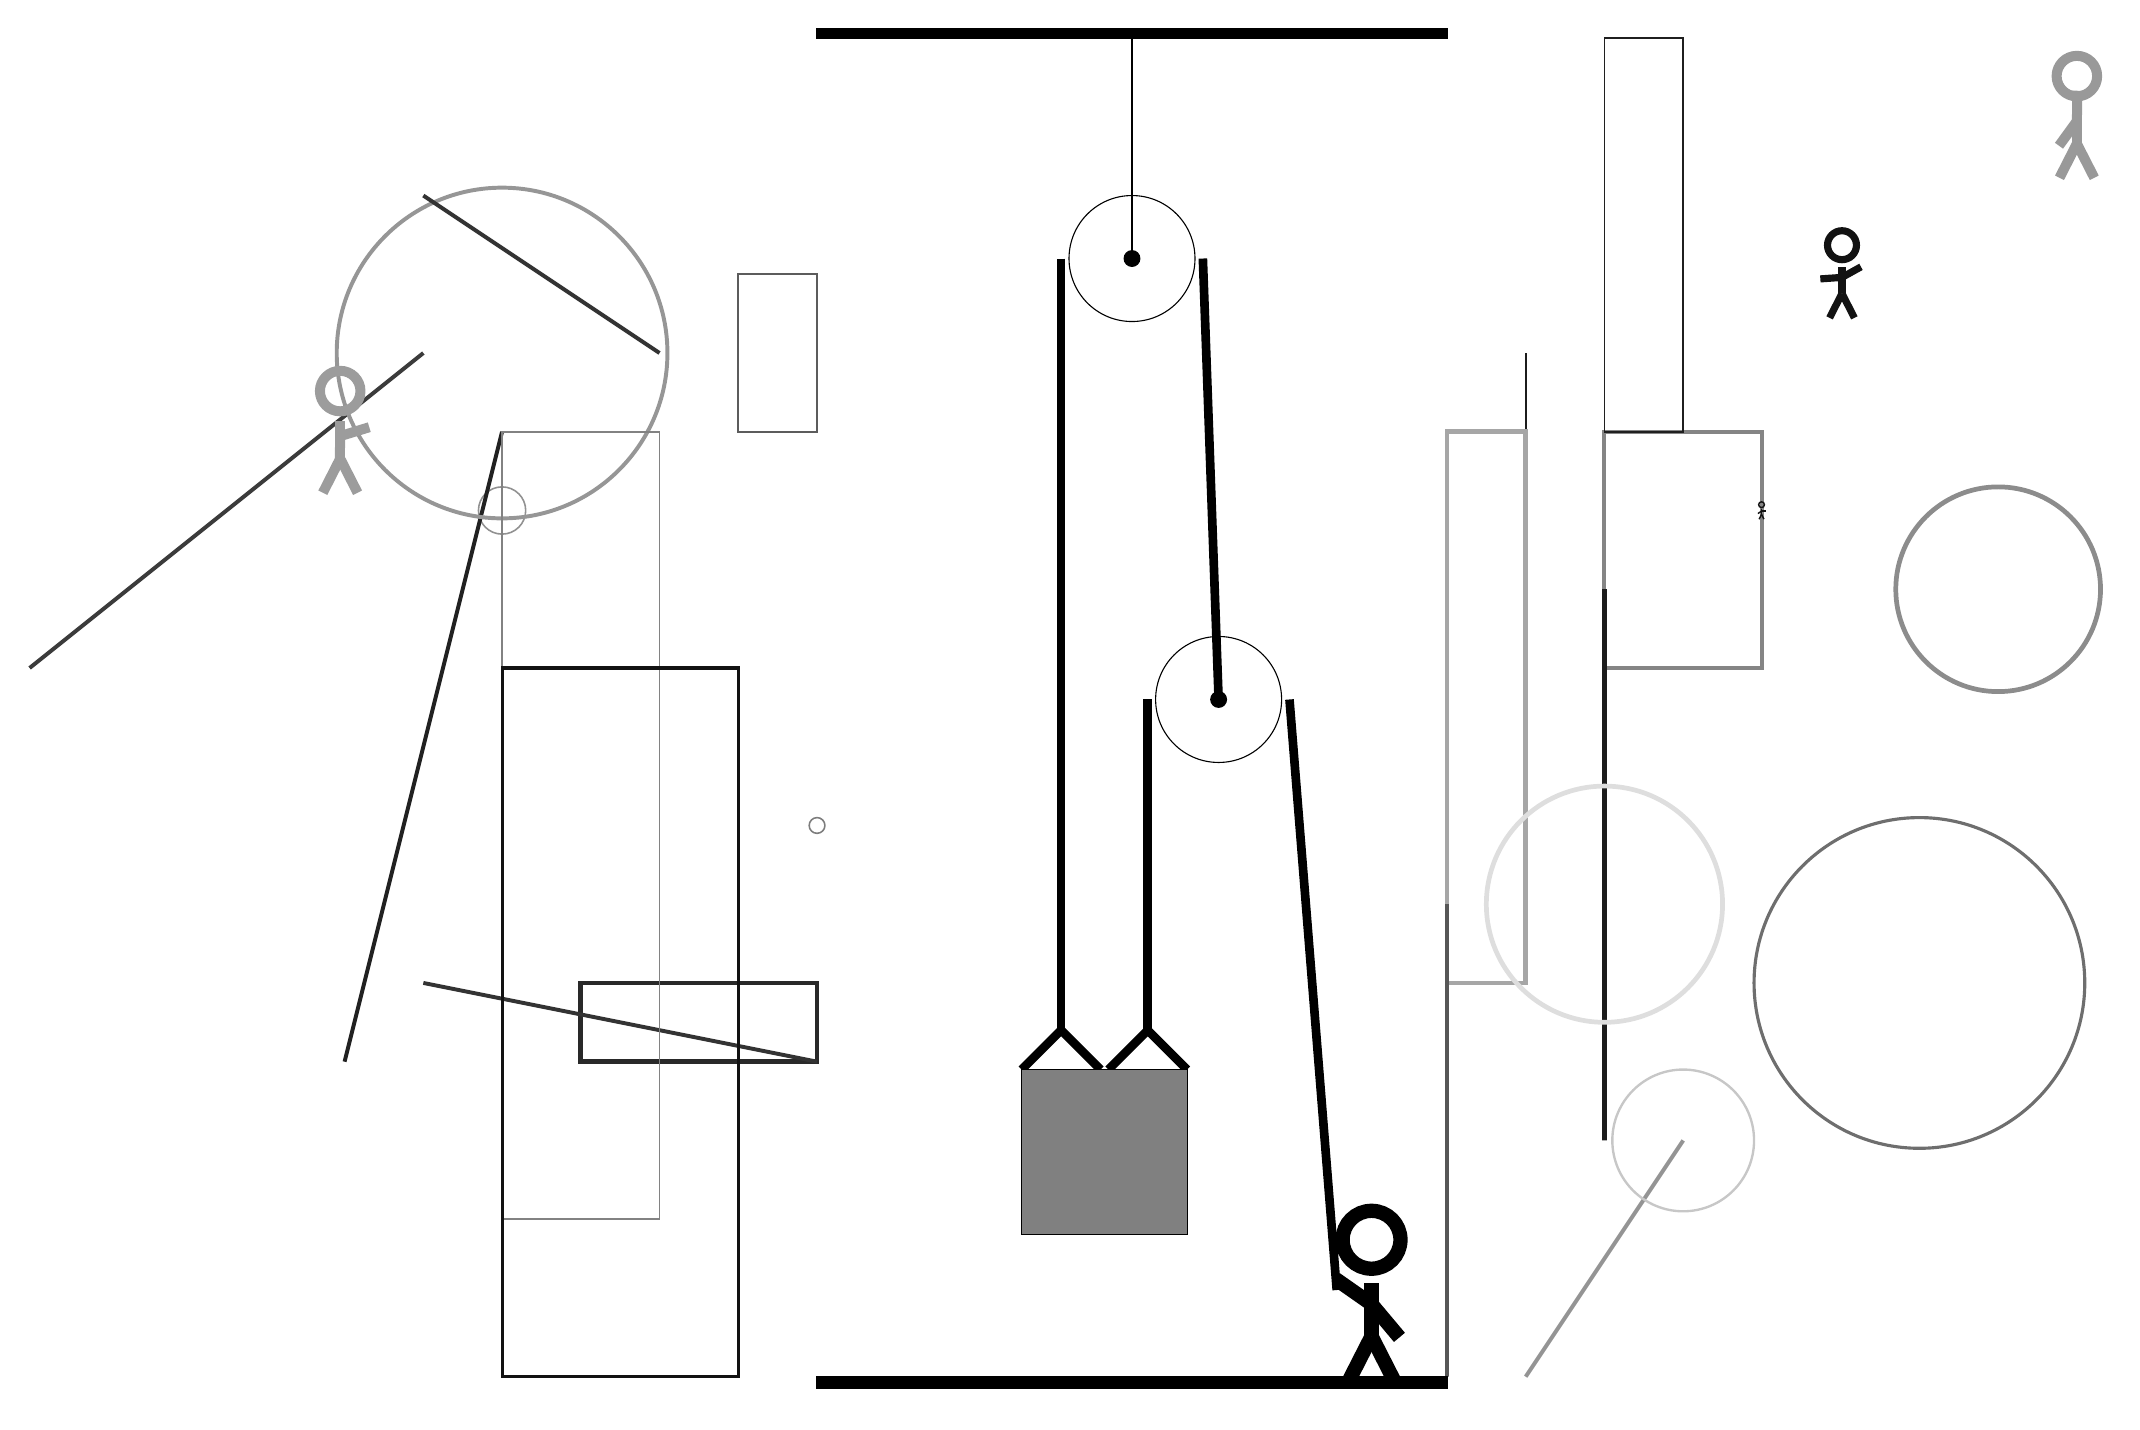
\begin{tikzpicture}
			%%%%% START %%%%%
			
			\draw[fill=black] (-2, 14) rectangle (6, 14.125);
			
			\draw (2, 11.2) circle (0.8);
			\draw[fill=black] (2, 11.2) circle (0.1);
			\draw[thick] (2, 11.2) -- (2, 14);
			
			\draw (3.1, 5.6) circle (0.8);
			\draw[fill=black] (3.1, 5.6) circle (0.1);
			
			\draw[line width=0.5mm, color=black!42](7, -3) -- (9, 0);
			
			\draw[line width=0.3mm, color=black!64] (-3, 11) rectangle (-2, 9);
			\draw[line width=0.6mm, color=black!84] (-2, 2) rectangle (-5, 1);
			\draw[line width=0.5mm, color=black!48] (8, 6) rectangle (10, 9);
			\draw [line width=0.4mm, color=black!57](12, 2) circle (2.1);
			\draw[line width=0.5mm, color=black!80](-2, 1) -- (-7, 2);
			\draw [line width=0.2mm, color=black!43](-6, 8) circle (0.3);
			\draw[line width=0.2mm, color=black!89] (7, 2) rectangle (7, 10);
			\draw[line width=0.7mm, color=black!89] (8, 7) rectangle (8, 0);
			\node[line width=0.2mm, color=black!40] at (14, 13) {\Strichmaxerl[7][54][89]};
			\draw [line width=0.3mm, color=black!22](9, 0) circle (0.9);
			\draw[line width=0.5mm, color=black!87](-6, 9) -- (-8, 1);
			\draw[line width=0.6mm, color=black!35] (7, 2) rectangle (6, 9);
			
			\draw[line width=0.5mm, color=black!77](-7, 10) -- (-12, 6);
			\draw [line width=0.6mm, color=black!45](13, 7) circle (1.3);
			\draw[line width=0.2mm, color=black!88] (8, 14) rectangle (9, 9);
			\node[line width=0.4mm, color=black!93] at (11, 11) {\Strichmaxerl[5][4][29]};
			
			\draw [line width=0.5mm, color=black!41](-6, 10) circle (2.1);
			\draw [line width=0.6mm, color=black!13](8, 3) circle (1.5);
			\draw[line width=0.2mm, color=black!49] (-4, 9) rectangle (-6, -1);
			\draw[line width=0.5mm, color=black!80](-7, 12) -- (-4, 10);
			\draw[line width=0.6mm, color=black!66] (6, 3) rectangle (6, -3);
			\draw [line width=0.2mm, color=black!51](-2, 4) circle (0.1);
			\node[line width=0.5mm, color=black!39] at (-8, 9) {\Strichmaxerl[7][89][17]};
			\node[line width=0.3mm, color=black!92] at (10, 8) {\Strichmaxerl[1][34][0]};
			\draw[line width=0.4mm, color=black!93] (-3, -3) rectangle (-6, 6);
			
			\draw[line width = 1.1mm]  (0.6, 0.9) -- (1.1, 1.4) -- (1.6, 0.9);
			\draw[line width = 1.1mm]  (1.7, 0.9) -- (2.2, 1.4) -- (2.7, 0.9);
			\draw[fill=black!50] (0.6, 0.9) rectangle (2.7, -1.2);
			
			\draw[line width = 1.1mm] (1.1, 11.2) -- (1.1, 1.4);
			\centerarc[line width = 1.1mm](2, 11.2)(0:180:0.9);
			\draw[line width = 1.1mm] (2.9, 11.2) -- (3.1, 5.6);
			\draw[line width = 1.1mm] (2.2, 5.6) -- (2.2, 1.4);
			\centerarc[line width = 1.1mm](3.1, 5.6)(0:180:0.9);
			\draw[line width = 1.1mm] (4.0, 5.6) -- (4.6, -1.9);
			
			\node at (5, -2) {\Strichmaxerl[10][-35][-50]};
			
			\draw[fill=black] (-2, -3) rectangle (6, -3.15);
			
			%%%%% END %%%%%
		\end{tikzpicture}
	\end{figure}	
\end{document}